\subsubsection{05.12.14}

\begin{enumerate}
	\item The time of beginning and ending of the meeting:
	16:00 - 20:00
	\item Purposes of the meeting:
	\begin{enumerate}
		\item To install П-shaped rib of rigidity.
		
		\item To measure the inner space of the robot and choose the optimal size of the bucket.
		
	\end{enumerate}
	\item Work that had been done:
	\begin{enumerate}
		\item П-shaped rib of rigidity had been installed.
		
		\begin{figure}[H]
			\begin{minipage}[h]{0.2\linewidth}
				\center  
			\end{minipage}
			\begin{minipage}[h]{0.6\linewidth}
				\center{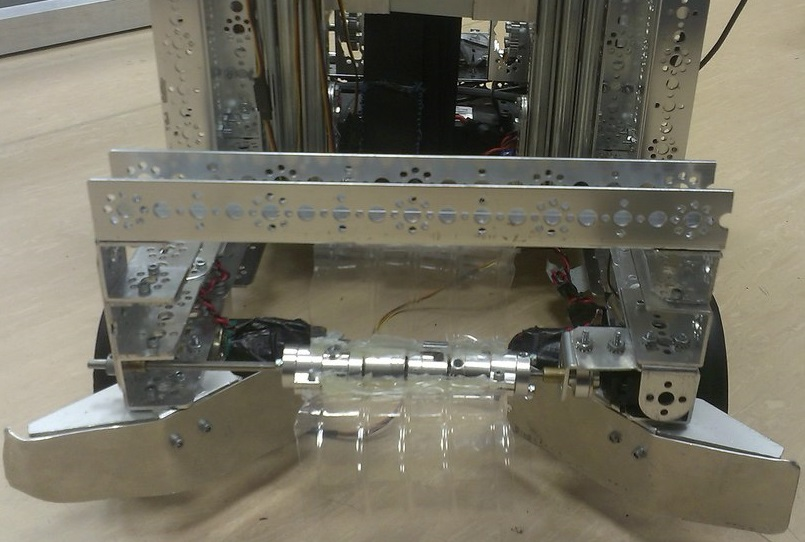
\includegraphics[scale=0.3]{days/05.12.14/images/01}}
				\caption{П-shaped rib of rigidity}
			\end{minipage}
		\end{figure}
		
		\item We measured the space allocated for bucket and chose optimal sizes for it.
		
		\item improved the program of autonomous period. Removed function that converted reading of encoder to centimeters. This increased the speed of the program and allowed the robot to accurately turn around and return to the parking zone.	  
		
	\end{enumerate}
	
	\item Results:  
	\begin{enumerate}
		\item П-shaped rib of rigidity installed.
		
		\item Program of autonomous period improved.
		
	\end{enumerate}
	
	\item Tasks for the next meetings:
	\begin{enumerate}
		\item To draw out the design for the new bucket.
		
		\item To choose and buy the material for the new bucket.
		
	\end{enumerate}     
\end{enumerate}
\fillpage